\documentclass[10pt, spanish, twocolumn]{article}
% --- Paquetes de Diseño Editorial NYT ---
\usepackage[utf8]{inputenc}
\usepackage[T1]{fontenc}
\usepackage{babel}
\usepackage{amsmath, amssymb, amsfonts}
\usepackage{libertinus}
\usepackage[default]{montserrat}
\usepackage{microtype}
\usepackage[margin=1.5cm, top=2.5cm, bottom=2cm, columnsep=0.8cm]{geometry}

% --- Gráficos y Diagramas ---
\usepackage{tikz}
\usepackage{pgfplots}
\pgfplotsset{compat=1.18}
\usetikzlibrary{patterns, arrows.meta, positioning, shapes.geometric}

% --- Paleta de Colores "The New York Times" ---
\usepackage{xcolor}
\definecolor{nytblack}{RGB}{18, 18, 18}
\definecolor{nytgray}{RGB}{120, 120, 120}
\definecolor{accentblue}{RGB}{50, 104, 145}
\definecolor{accentred}{RGB}{204, 0, 0}
\definecolor{accentgreen}{RGB}{0, 128, 96}

% --- Ingeniería de Títulos Estilo "Magazine" ---
\usepackage[explicit]{titlesec}
\titleformat{\section}
  {\normalfont\bfseries\sffamily\Large\color{nytblack}}
  {}{0pt}{\MakeUppercase{#1}}[{\color{nytblack}\titlerule[1.5pt]}]
\titleformat{\subsection}
  {\normalfont\bfseries\sffamily\normalsize\color{accentblue}}
  {}{0pt}{#1}

% --- Letra Capital Gigante ---
\usepackage{lettrine}
\renewcommand{\LettrineFontSpec}{\itshape\color{nytblack}}

% --- Caja de "The Daily Brief" ---
\usepackage[most]{tcolorbox}
\newtcolorbox{briefbox}[1]{
    enhanced,
    colback=white,
    colframe=nytblack!20,
    arc=0mm,
    boxrule=0.5pt,
    leftrule=3pt,
    fonttitle=\sffamily\bfseries\small,
    coltitle=nytblack,
    title=#1,
    attach title to upper,
    after title={ \textbar \ },
    drop fuzzy shadow
}

\newtcolorbox{theorembox}[1]{
    enhanced,
    colback=accentblue!5,
    colframe=accentblue,
    arc=0mm,
    boxrule=1pt,
    fonttitle=\sffamily\bfseries\small,
    coltitle=white,
    title=#1,
    attach title to upper={},
    drop fuzzy shadow
}

\newtcolorbox{examplebox}[1]{
    enhanced,
    colback=accentgreen!5,
    colframe=accentgreen!80,
    arc=0mm,
    boxrule=0.8pt,
    fonttitle=\sffamily\bfseries\small,
    coltitle=nytblack,
    title=#1,
    attach title to upper,
    after title={ \\ },
}

% --- Header Estilo Periódico ---
\usepackage{fancyhdr}
\pagestyle{fancy}
\fancyhf{}
\fancyhead[C]{\small\sffamily\textbf{THE SCIENCE TIMES} \quad \textbar \quad \textbf{MATHEMATISCHE GRUNDLAGEN}}
\fancyfoot[C]{\thepage}
\renewcommand{\headrulewidth}{0.8pt}

\begin{document}

% --- Portada de Sección Mega Increíble ---
\twocolumn[
  \begin{center}
    \vspace*{-1cm}
    {\fontsize{50}{55}\selectfont\textbf{Fundamentos}} \\
    {\fontsize{42}{47}\selectfont\textbf{Matemáticos}} \\
    \vspace{0.4cm}
    {\LARGE \textit{El lenguaje silencioso que construye la realidad científica.}} \\
    \vspace{0.5cm}
    {\large \sffamily Por Emanuel Quintana Silva | UPTC} \\
    \vspace{0.8cm}
    \begin{minipage}{0.9\textwidth}
        \centering
        \hrule height 1.2pt \vspace{2pt} \hrule height 0.5pt
        \vspace{0.2cm}
        \small\sffamily \textbf{INVESTIGACIÓN ESPECIAL} \quad $\bullet$ \quad PAPULA BAND 1 \quad $\bullet$ \quad ENERO 2026
        \vspace{0.2cm}
        \hrule height 0.5pt \vspace{2pt} \hrule height 1.2pt
    \end{minipage}
    \vspace{1.2cm}
  \end{center}
]

% --- Inicio del Texto ---
\lettrine[lines=3, findent=2pt, nindent=0pt]{L}{a} transición del pensamiento escolar a la estructura de las disciplinas científicas superiores requiere más que fórmulas; exige un marco lógico riguroso. Basado en la obra monumental de Lothar Papula, \textit{Mathematik für Ingenieure und Naturwissenschaftler}, la teoría de conjuntos se presenta no como un tema aislado, sino como el \textbf{átomo de la lógica moderna}.

\section{Ontología de la Unidad}

Un conjunto es la agrupación de objetos bien diferenciados en una unidad conceptual. Esta definición, aparentemente simple, es la piedra angular del análisis matemático moderno y constituye el fundamento sobre el cual se erigen todas las estructuras algebraicas superiores.

\begin{briefbox}{PRINCIPIO FUNDAMENTAL}
    Para que un sistema se considere un conjunto válido, la pertenencia debe ser absoluta y verificable. No existen espacios para la ambigüedad: un elemento pertenece ($\in$) o es completamente ajeno ($\notin$) al conjunto.
\end{briefbox}

\subsection{Características Esenciales}

Los elementos que conforman un conjunto deben cumplir dos condiciones ineludibles: ser \textbf{distintos entre sí} y estar \textbf{bien diferenciados}. El orden en que se enumeran carece de relevancia lógica, estableciendo así una estructura simétrica fundamental.

\section{Dualidad de Representación}

En el diseño científico riguroso, la claridad representacional es el valor supremo. Los conjuntos se manifiestan en dos formas complementarias, cada una con aplicaciones específicas según la naturaleza del problema.

\subsection{El Método Descriptivo}

Define la esencia mediante una propiedad característica. Es el método obligatorio para sistemas infinitos donde la enumeración resulta imposible.

\[ M = \{x \mid x \text{ satisface la propiedad } E \} \]

Este método utiliza el poder del lenguaje lógico para capturar la esencia abstracta del conjunto. Por ejemplo, el conjunto de números naturales se define como $\mathbb{N} = \{x \mid x \text{ es entero y } x \geq 0\}$.

\subsection{El Método Enumerativo}

Listado directo de elementos. Representa la evidencia tangible y concreta de la colección finita.

\[ M_3 = \{ -3, -2, -1, 0, 1, 2, 3 \} \]

La enumeración explícita elimina toda ambigüedad y permite verificación inmediata de pertenencia.

\section{Operaciones Fundamentales}

Las operaciones entre conjuntos (Mengenoperationen) constituyen el álgebra fundamental que permite construir estructuras matemáticas complejas a partir de unidades simples.

\subsection{Intersección: La Lógica del "Y"}

La \textbf{intersección} de dos conjuntos $A$ y $B$, denotada $A \cap B$, representa el conjunto de elementos que pertenecen simultáneamente a ambos.

\begin{theorembox}{DEFINICIÓN FORMAL}
\[ A \cap B = \{x \mid x \in A \text{ y } x \in B\} \]
\end{theorembox}

\begin{examplebox}{APLICACIÓN TÉCNICA}
Al resolver el sistema de inecuaciones:
\begin{align*}
2x - 4 &> 0 \quad \Rightarrow \quad x > 2 \\
x &< 3
\end{align*}
La solución es la intersección: $L = \{x \mid 2 < x < 3\} = (2,3)$
\end{examplebox}

\begin{center}
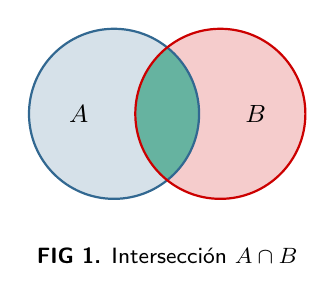
\begin{tikzpicture}[scale=0.9]
    % Diagrama de Venn para Intersección
    \begin{scope}
        \fill[accentblue!20] (0,0) circle (1.2cm);
        \fill[accentred!20] (1.5,0) circle (1.2cm);
        \begin{scope}
            \clip (0,0) circle (1.2cm);
            \fill[accentgreen!60] (1.5,0) circle (1.2cm);
        \end{scope}
        \draw[accentblue, thick] (0,0) circle (1.2cm);
        \draw[accentred, thick] (1.5,0) circle (1.2cm);
        \node at (-0.5, 0) {\small\sffamily $A$};
        \node at (2, 0) {\small\sffamily $B$};
        \node at (0.75, -2) {\footnotesize\sffamily\textbf{FIG 1.} Intersección $A \cap B$};
    \end{scope}
\end{tikzpicture}
\end{center}

\subsection{Unión: La Lógica Inclusiva del "O"}

La \textbf{unión} de conjuntos $A$ y $B$, simbolizada $A \cup B$, agrupa todos los elementos que pertenecen al menos a uno de los conjuntos.

\begin{theorembox}{DEFINICIÓN FORMAL}
\[ A \cup B = \{x \mid x \in A \text{ o } x \in B\} \]
\end{theorembox}

El "o" lógico es \textbf{inclusivo}: los elementos comunes a ambos conjuntos forman parte integral de la unión.

\begin{examplebox}{EJEMPLO NUMÉRICO}
Sean $A = \{1, 2, 3, 4\}$ y $B = \{1, 5, 6, 7\}$. Entonces:
\[ A \cup B = \{1, 2, 3, 4, 5, 6, 7\} \]
\end{examplebox}

\begin{center}
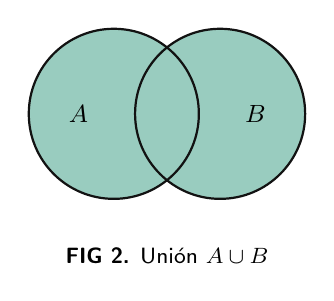
\begin{tikzpicture}[scale=0.9]
    \fill[accentgreen!40] (0,0) circle (1.2cm);
    \fill[accentgreen!40] (1.5,0) circle (1.2cm);
    \draw[nytblack, thick] (0,0) circle (1.2cm);
    \draw[nytblack, thick] (1.5,0) circle (1.2cm);
    \node at (-0.5, 0) {\small\sffamily $A$};
    \node at (2, 0) {\small\sffamily $B$};
    \node at (0.75, -2) {\footnotesize\sffamily\textbf{FIG 2.} Unión $A \cup B$};
\end{tikzpicture}
\end{center}

\subsection{Diferencia: El Operador de Exclusión}

La \textbf{diferencia} $A \setminus B$ (leído "$A$ sin $B$") contiene exclusivamente los elementos de $A$ que no pertenecen a $B$.

\begin{theorembox}{DEFINICIÓN FORMAL}
\[ A \setminus B = \{x \mid x \in A \text{ y } x \notin B\} \]
\end{theorembox}

\begin{examplebox}{CONSTRUCCIÓN DE CONJUNTOS DERIVADOS}
Los números naturales positivos se definen mediante diferencia:
\[ \mathbb{N}^* = \mathbb{N} \setminus \{0\} = \{1, 2, 3, \dots\} \]
\end{examplebox}

\section{Relaciones de Inclusión}

\begin{center}
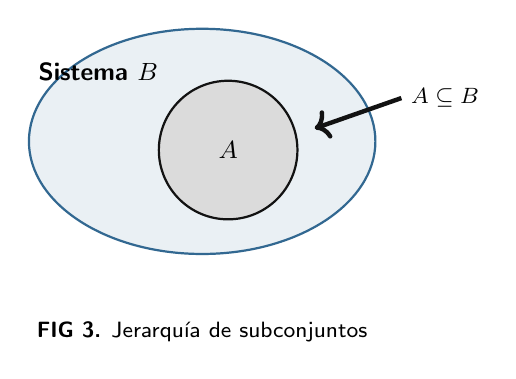
\begin{tikzpicture}[scale=1.1]
    \fill[accentblue!10] (0,0) ellipse (2cm and 1.3cm);
    \draw[accentblue, thick] (0,0) ellipse (2cm and 1.3cm);
    \fill[nytblack!15] (0.3,-0.1) circle (0.8cm);
    \draw[nytblack, thick] (0.3,-0.1) circle (0.8cm);
    
    \node at (-1.2, 0.8) {\small\sffamily\textbf{Sistema $B$}};
    \node at (0.3, -0.1) {\small\sffamily\textbf{$A$}};
    
    \draw[->, nytblack, ultra thick] (2.3,0.5) -- (1.3,0.15);
    \node[right] at (2.3,0.5) {\footnotesize\sffamily $A \subseteq B$};
    
    \node at (0, -2.2) {\footnotesize\sffamily\textbf{FIG 3.} Jerarquía de subconjuntos};
\end{tikzpicture}
\end{center}

\section{Identidad y el Vacío}

La igualdad de conjuntos ($A=B$) ocurre únicamente cuando poseen exactamente los mismos elementos. El \textbf{conjunto vacío} ($\emptyset$) es, paradójicamente, el concepto más fundamental: permite definir sistemas sin soluciones reales, asegurando que la lógica matemática nunca colapse.

\section{Los Números Reales}

\lettrine[lines=2]{E}{l} conjunto $\mathbb{R}$ constituye la columna vertebral de todo el análisis matemático aplicado. Representa la completitud numérica absoluta.

\subsection{Estructura y Representación}

Los números reales incluyen tres categorías:
\begin{enumerate}
\item Decimales finitos (incluyen enteros)
\item Decimales infinitos periódicos (números racionales)
\item Decimales infinitos no periódicos (números irracionales)
\end{enumerate}

\begin{briefbox}{CORRESPONDENCIA BIUNÍVOCA}
Existe una relación uno a uno entre los números reales y los puntos de la recta numérica dirigida, estableciendo una \textbf{geometrización} completa de la aritmética.
\end{briefbox}

\begin{center}
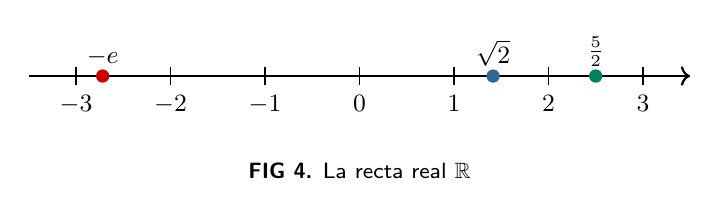
\begin{tikzpicture}[scale=1.2]
    \draw[->, thick] (-3.5,0) -- (3.5,0);
    \foreach \x in {-3,-2,-1,0,1,2,3}
        \draw (\x,0.1) -- (\x,-0.1) node[below] {\small $\x$};
    
    \fill[accentblue] (1.414,0) circle (2pt);
    \node[above] at (1.414,0) {\small $\sqrt{2}$};
    
    \fill[accentred] (-2.718,0) circle (2pt);
    \node[above] at (-2.718,0) {\small $-e$};
    
    \fill[accentgreen] (2.5,0) circle (2pt);
    \node[above] at (2.5,0) {\small $\frac{5}{2}$};
    
    \node at (0, -1) {\footnotesize\sffamily\textbf{FIG 4.} La recta real $\mathbb{R}$};
\end{tikzpicture}
\end{center}

\subsection{Leyes Estructurales}

El sistema $\mathbb{R}$ está gobernado por tres leyes algebraicas fundamentales:

\begin{theorembox}{LEYES CONMUTATIVAS}
\[ a + b = b + a \quad ; \quad a \cdot b = b \cdot a \]
El orden de operación no altera el resultado.
\end{theorembox}

\begin{theorembox}{LEYES ASOCIATIVAS}
\[ a + (b + c) = (a + b) + c \quad ; \quad a(bc) = (ab)c \]
La agrupación no modifica el valor final.
\end{theorembox}

\begin{theorembox}{LEY DISTRIBUTIVA}
\[ a(b + c) = ab + ac \]
Conecta multiplicación con adición, fundamento del álgebra.
\end{theorembox}

\section{Orden y Desigualdades}

\subsection{Anordnung der Zahlen}

Para cualquier par $a, b \in \mathbb{R}$, se cumple exactamente una de tres relaciones: $a < b$, $a = b$, o $a > b$. Esta tricotomía es la esencia del orden total.

\textbf{Interpretación Geométrica:}
\begin{itemize}
\item $a < b$: El punto $a$ está a la izquierda de $b$
\item $a > b$: El punto $a$ está a la derecha de $b$
\item $a = b$: Ambos puntos coinciden
\end{itemize}

\subsection{Transformaciones de Inecuaciones}

Las inecuaciones se resuelven mediante transformaciones equivalentes:

\begin{examplebox}{REGLAS DE TRANSFORMACIÓN}
\textbf{1. Adición/Sustracción:} Se puede sumar o restar cualquier término en ambos lados sin cambiar el signo de desigualdad.

\textbf{2. Multiplicación por positivos:} Si $c > 0$, entonces $a < b \Rightarrow ac < bc$.

\textbf{3. Multiplicación por negativos:} Si $c < 0$, entonces $a < b \Rightarrow ac > bc$ (el signo se invierte).
\end{examplebox}

\subsection{Valor Absoluto: Distancia Numérica}

El \textbf{valor absoluto} $|a|$ representa la distancia del número $a$ al origen en la recta numérica.

\begin{theorembox}{DEFINICIÓN POR CASOS}
\[ |a| = \begin{cases} 
a & \text{si } a > 0 \\
0 & \text{si } a = 0 \\
-a & \text{si } a < 0
\end{cases} \]
\end{theorembox}

\textbf{Propiedad Métrica:} $|x - a|$ mide la distancia entre $x$ y $a$.

\begin{center}
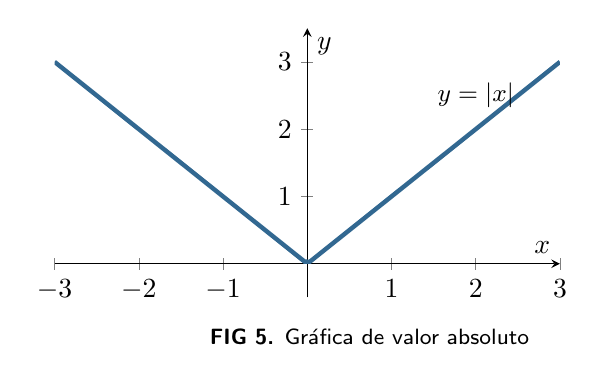
\begin{tikzpicture}[scale=1]
    \begin{axis}[
        axis lines=middle,
        xlabel={$x$},
        ylabel={$y$},
        domain=-3:3,
        samples=100,
        width=8cm,
        height=5cm,
        ymin=-0.5, ymax=3.5
    ]
    \addplot[accentblue, ultra thick] {abs(x)};
    \node at (axis cs: 2,2.5) {\small $y = |x|$};
    \end{axis}
    \node at (4, -0.5) {\footnotesize\sffamily\textbf{FIG 5.} Gráfica de valor absoluto};
\end{tikzpicture}
\end{center}

\section{Teoría de Ecuaciones}

\subsection{Ecuaciones Lineales}

La forma canónica $ax + b = 0$ ($a \neq 0$) posee exactamente una solución:
\[ x = -\frac{b}{a} \]

\subsection{Ecuaciones Cuadráticas}

La forma general $ax^2 + bx + c = 0$ se normaliza a $x^2 + px + q = 0$.

\begin{theorembox}{FÓRMULA $p,q$}
\[ x_{1,2} = -\frac{p}{2} \pm \sqrt{\left(\frac{p}{2}\right)^2 - q} \]
\end{theorembox}

El \textbf{discriminante} $D = (p/2)^2 - q$ determina la naturaleza de las soluciones:

\begin{center}
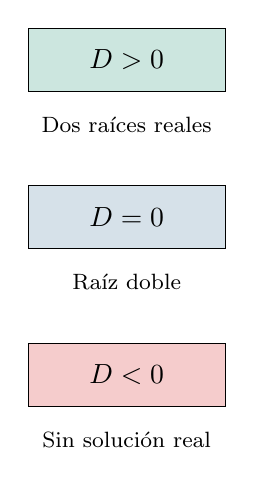
\begin{tikzpicture}
    \node[draw, fill=accentgreen!20, rectangle, minimum width=2.5cm, minimum height=0.8cm] at (0,2) {$D > 0$};
    \node[below] at (0,1.4) {\footnotesize Dos raíces reales};
    
    \node[draw, fill=accentblue!20, rectangle, minimum width=2.5cm, minimum height=0.8cm] at (0,0) {$D = 0$};
    \node[below] at (0,-0.6) {\footnotesize Raíz doble};
    
    \node[draw, fill=accentred!20, rectangle, minimum width=2.5cm, minimum height=0.8cm] at (0,-2) {$D < 0$};
    \node[below] at (0,-2.6) {\footnotesize Sin solución real};
\end{tikzpicture}
\end{center}

\subsection{Ecuaciones de Grado Superior}

\textbf{Teorema Fundamental del Álgebra:} Una ecuación de grado $n$ posee como máximo $n$ soluciones reales.

\begin{examplebox}{ECUACIONES BICUADRÁTICAS}
Para $ax^4 + bx^2 + c = 0$, se aplica la sustitución $u = x^2$, convirtiéndola en ecuación cuadrática en $u$. Posteriormente se obtienen las raíces mediante $x = \pm\sqrt{u}$.
\end{examplebox}

\subsection{Esquema de Horner}

Método eficiente para evaluar polinomios y realizar división sintética. Si $x_1$ es raíz conocida de $P(x)$, el esquema permite dividir por $(x - x_1)$ y reducir el grado del polinomio.

\subsection{Ecuaciones Irracionales}

Contienen la incógnita bajo radicales. El método consiste en aislar el radical y elevar a la potencia adecuada.

\begin{briefbox}{ADVERTENCIA CRÍTICA}
Elevar al cuadrado NO es transformación equivalente. Pueden aparecer \textbf{soluciones falsas} (Scheinlösungen). La verificación en la ecuación original es \textbf{obligatoria}.
\end{briefbox}

\subsection{Ecuaciones con Valor Absoluto}

Se resuelven mediante \textbf{distinción de casos} (Fallunterscheidung), analizando los intervalos donde el argumento del valor absoluto es positivo o negativo.

\section{Sistemas de Ecuaciones Lineales}

Un sistema de $m$ ecuaciones con $n$ incógnitas se representa matricialmente como:
\[ A\tilde{x} = \tilde{c} \]

\subsection{Algoritmo de Gauss}

Método de eliminación sistemática que transforma el sistema en forma escalonada mediante operaciones elementales:
\begin{enumerate}
\item Intercambio de ecuaciones
\item Multiplicación de ecuación por constante no nula
\item Adición de múltiplo de una ecuación a otra
\end{enumerate}

\begin{theorembox}{CASOS DE SOLUCIÓN}
\textbf{1. Solución única:} Sistema determinado (matriz regular)

\textbf{2. Infinitas soluciones:} Sistema indeterminado (solución paramétrica)

\textbf{3. Sin solución:} Sistema incompatible (contradicción lógica)
\end{theorembox}

\subsection{Regla de Cramer}

Para sistemas con matriz cuadrada regular ($\det(A) \neq 0$):
\[ x_i = \frac{\det(A_i)}{\det(A)} \]
donde $A_i$ es la matriz $A$ con la columna $i$ reemplazada por el vector $\tilde{c}$.

\section{Métodos Numéricos}

\subsection{Método de Newton}

Para ecuaciones trascendentes sin solución analítica, el método de Newton (Tangentenverfahren) proporciona aproximaciones iterativas:

\begin{theorembox}{FÓRMULA ITERATIVA}
\[ x_{n+1} = x_n - \frac{f(x_n)}{f'(x_n)} \]
\end{theorembox}

La convergencia es cuadrática cerca de la raíz, garantizando precisión exponencial.

\begin{center}
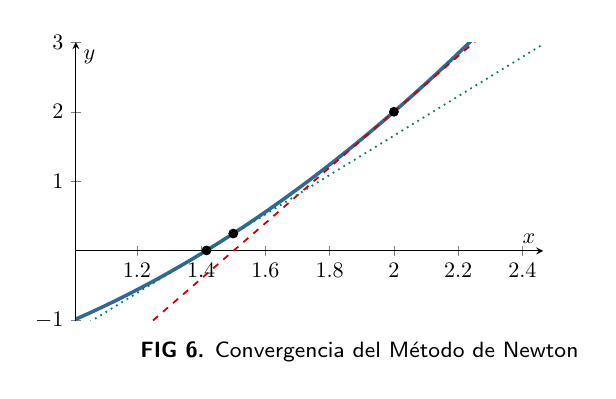
\begin{tikzpicture}[scale=0.8]
    \begin{axis}[
        axis lines=middle,
        xlabel={$x$},
        ylabel={$y$},
        domain=0:4,
        samples=100,
        width=9cm,
        height=6cm,
        ymin=-1, ymax=3
    ]
    \addplot[accentblue, ultra thick] {x^2 - 2};
    \addplot[accentred, dashed, thick] {4*x - 6};
    \addplot[accentgreen, dotted, thick] {2.8284*x - 4};
    
    \addplot[mark=*, only marks, mark size=2pt] coordinates {(2,2) (1.5,0.25) (1.4167,0.0069)};
    
    \node at (axis cs: 3,1.5) {\small $f(x) = x^2 - 2$};
    \end{axis}
    \node at (4.5, -0.5) {\footnotesize\sffamily\textbf{FIG 6.} Convergencia del Método de Newton};
\end{tikzpicture}
\end{center}

\section{Conclusión Técnica}

Los fundamentos matemáticos presentados constituyen el andamiaje conceptual sobre el cual se erigen todas las disciplinas científico-técnicas. La teoría de conjuntos proporciona el lenguaje, los números reales la métrica, y las ecuaciones el mecanismo de modelado.

En el rigor de la ingeniería moderna, según las enseñanzas de Papula, solo la precisión lógica y la coherencia estructural garantizan resultados confiables. Los elementos deben ser distintos, el orden irrelevante, y la pertenencia absoluta.

\vspace{0.5cm}
\begin{briefbox}{REFERENCIAS}
\textbf{Fuente Principal:} Papula, L. (2024). \textit{Mathematik für Ingenieure und Naturwissenschaftler, Band 1} (16ª ed.). Springer Vieweg. ISBN 978-3-658-45801-0.

\textbf{Investigador:} Emanuel Quintana Silva, Economista en formación (UPTC). Especialización en Econometría Computacional. ORCID: 0009-0006-8419-2805.
\end{briefbox}

\vspace{1cm}
\begin{center}
    \color{nytgray}
    \rule{0.4\linewidth}{0.6pt} \\
    \vspace{0.15cm}
    \small\sffamily PRÓXIMA EDICIÓN: ÁLGEBRA VECTORIAL Y GEOMETRÍA ANALÍTICA
    \vspace{0.1cm}
    
    \rule{0.4\linewidth}{0.6pt}
\end{center}

\end{document}